\section{Tests and Evaluation}
\label{sec:tests}

\subsection{Testing Strategy}

The metamodels are tested by instantiating them. Accepted models show that the
metamodels represent the intended deployments, and rejected models show that
the constraints reject invalid ones.

\begin{itemize}
  \item \textbf{Accepted models.} Five project documents and one platform
    document instantiate the source metamodel
    (Section~\ref{sec:examplemodels}). They are modelled on applications of the
    existing configuration. One hand-written resolved model instantiates the
    target metamodel.
  \item \textbf{Rejected models.} Thirty-three models each break one rule
    (Section~\ref{sec:rejectedmodels}).
  \item \textbf{Automated checks.} Every build parses each accepted and
    rejected model with the Xtext grammars, validates it against the OCL
    constraints, and compares the outcome with a committed expected result: the
    parsed model for an accepted model, and the codes and object paths for a
    rejected one (Section~\ref{sec:implementation}). A change to a metamodel,
    grammar or constraint that alters any outcome fails the build. Further tests
    check the hand-written resolved model against the target metamodel: it
    validates, a prepare process has no \texttt{cutover}, only a blue/green
    application has a release gate, and the path plan assigns a path to every
    file of the expected output.
  \item \textbf{Manual checks.} The hand-in holds each model as YAML and XMI.
    Validating an XMI in Eclipse repeats the check (Appendix~\ref{sec:handin}).
\end{itemize}

\subsection{Example Models}
\label{sec:examplemodels}

Table~\ref{tab:examples} lists five accepted source models.
Appendix~\ref{sec:handin} gives their paths.

\begin{table}[!htbp]
\centering
\small
\begin{tabular}{>{\raggedright\arraybackslash}p{0.16\linewidth}>{\raggedright\arraybackslash}p{0.76\linewidth}}
\hline
\textbf{Example} & \textbf{What it tests} \\
\hline
minimal & The smallest complete model: one project, one application, one
  process, and only required values. \\
auth & Two \texttt{continuous} processes in one application, so the release gate has two
  members and its deadline is the maximum over the members. It also has a
  managed migration, because the application uses a database. \\
data & Several applications in one project share a namespace. Each volume's
  durability class determines its backup plan. \\
knowledge & Two applications with different \texttt{cutover} values: a
  \texttt{continuous} API that migrates the project database with a changelog,
  and an \texttt{interrupted} worker
  with a volume. The worker has no migration. The example also has dependencies,
  shared secrets and routes with different audiences. \\
delivery & Two applications of the delivery machinery: Flagger and the release gate.
  Their processes are \texttt{continuous} but are updated in place instead of
  switched blue/green, because the release gate cannot control its own
  release. \\
\hline
\end{tabular}
\caption{The Example Models and What Each Tests}
\label{tab:examples}
\end{table}

Appendix~\ref{sec:appendix} describes two accepted examples and one rejected
case in more detail.

\subsubsection{The Minimal Model}

The minimal model omits rollout strategy, resource limits, security context,
labels, selector, namespace, probe timings and instance count. Platform rules
derive these values or reject omissions that cannot be derived.

\subsubsection{A Resolved Model as a Deployment View}

Figure~\ref{fig:deploymentview} shows the \texttt{knowledge} resolved model as a
deployment view (Section~\ref{sec:design}). It shows two processes on their
machines, a volume, the edge tier, a hostname and two platform services.

\begin{figure}[!htbp]
\centering
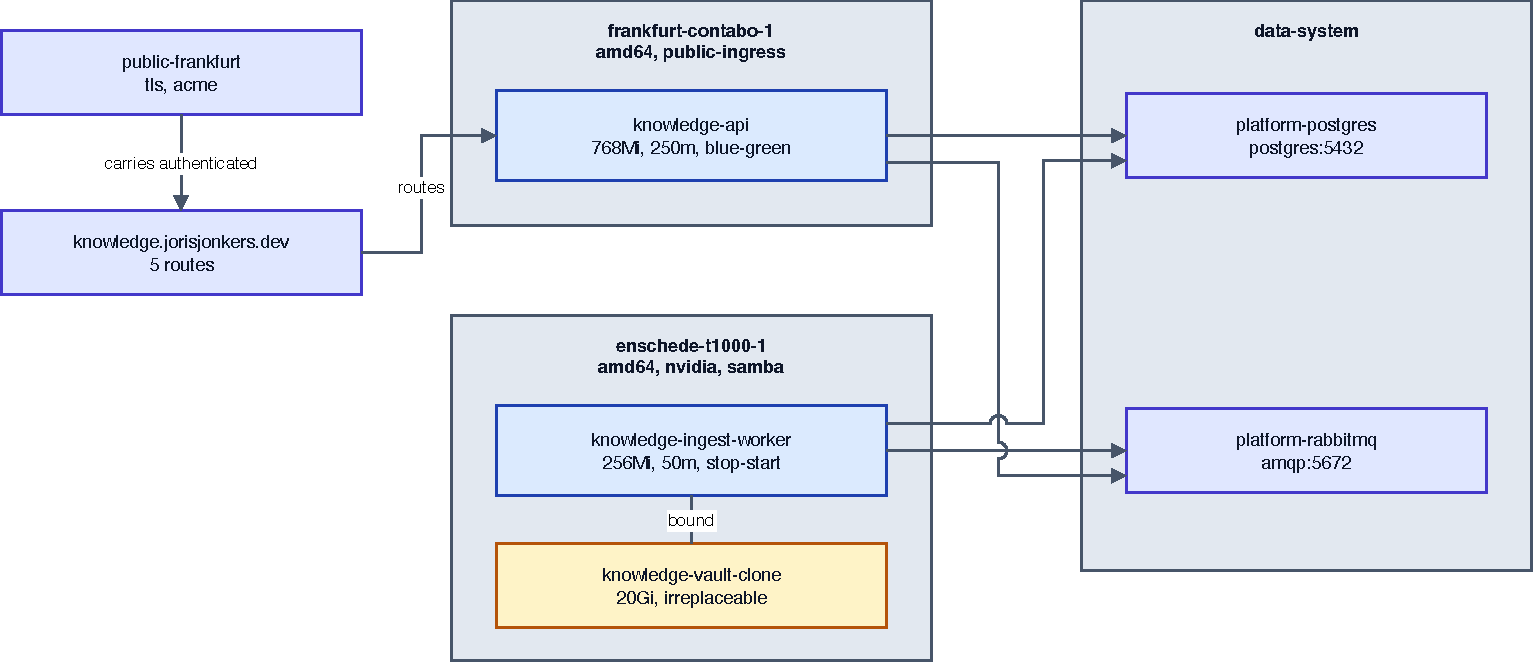
\includegraphics[width=\linewidth, keepaspectratio]{Figures/deployment-view}
\caption{The knowledge Example's Resolved Model as a Deployment View}
\label{fig:deploymentview}
\end{figure}

\subsubsection{Example Target Models}

The hand-written \texttt{minimal.resolveddeployment} is the expected Task 2
output and an input for testing Task 3 templates.

\subsection{Rejected Models}
\label{sec:rejectedmodels}

The archive has 33 rejected models: 18 single project files and 15 pairs of a
platform document and a project file. Together they cover all 28 constraint
codes and the four codes of unresolved names. Each file of a pair is valid on
its own. Validating a rejected model reports the violated invariant, whose name
is the code (Appendix~\ref{sec:appendix-refused}). The archive's
\texttt{refusals/README.md} says which file holds each error, and
Appendix~\ref{sec:allconstraints} says what each code rejects.

\subsection{Evaluation Against the Purpose}

Table~\ref{tab:evaluation} relates each observation of
Section~\ref{sec:observations} to the part of the metamodels that addresses it,
and to the models that show it.

\begin{table}[!htbp]
\centering
\footnotesize
\begin{tabular}{>{\raggedright\arraybackslash}p{0.22\linewidth}>{\raggedright\arraybackslash}p{0.42\linewidth}>{\raggedright\arraybackslash}p{0.26\linewidth}}
\hline
\textbf{Observation} & \textbf{How the metamodels address it} & \textbf{Shown by} \\
\hline
Repeated values & A hostname is declared once, on an \texttt{Exposure}, and a port once, on a \texttt{Surface}. Routes and dependencies refer to them by name. & All examples; \texttt{unknown-surface} \\
Repeated derivations & The resolved model derives switchover, probe timings and deadline from the declared \texttt{cutover} and startup budget. & Table~\ref{tab:minimal-trace} \\
Mechanisms instead of requirements & \texttt{cutover}, placement and writable paths state requirements. \texttt{E\_CUTOVER\_UNHONOURABLE} rejects a \texttt{continuous} process with a volume only one pod can mount. & \texttt{cutover-continuous-over-rwo} \\
Shared values & The platform document holds them, and constraints check a project document against it. & The 15 rejected pairs \\
\hline
\end{tabular}
\caption{Observations, How the Metamodels Address Them, and the Models That Show It}
\label{tab:evaluation}
\end{table}

\subsection{Limitations}
\label{sec:limitations}

\begin{itemize}
  \item The constraints embedded in the archive's \texttt{project-intent.ecore}
    do not see a second document. A rejected pair is reproduced in Eclipse only
    with both XMI files and \texttt{project-intent.ocl} loaded.
  \item Only the minimal example has a resolved model, written by hand. The
    resolved models of the other examples come from the Task 2 transformation,
    so the target metamodel is tested less than the source metamodel.
  \item Memory and CPU are checked per machine, not summed across the cluster
    (Section~\ref{sec:sharedvalues}).
  \item Constraints over all project documents at once, such as unique
    application identifiers, are not in OCL.
  \item The concrete syntax covers only the YAML subset of the existing
    configuration.
  \item The platform example is parsed without the project documents that
    declare the applications it refers to, so six references in its XMI stay
    unresolved.
  \item Figure~\ref{fig:projectdocument} leaves out two dependencies of
    \texttt{Placeholder}, to \texttt{Grant} and \texttt{Exposure}.
\end{itemize}

\subsection{Reflection}

Separating the authored and the resolved model kept both metamodels small. The
source metamodel holds only what an author must write, and the target metamodel
holds only the platform's decisions. Enumerations, and naming each invariant
after its code, made the rejected models easy to check, because each reports one
known code. The constraints across documents were the hardest part: OCL
evaluates one object at a time, so a rule between a platform document and a
project file needs \texttt{allInstances()} and a guard, and Eclipse evaluates
such rules only with the OCL document loaded. Without overrides, a wrong
derivation rule affects every process of its kind, so the Task 2 transformation
needs tests for each rule.
